\documentclass[8pt,a4paper]{article}
\usepackage[utf8]{inputenc}
\usepackage{graphicx}
\graphicspath{ {./images/} }

\usepackage{color}   
\usepackage{hyperref}
\usepackage{listings}
\usepackage[utf8]{inputenc}
\usepackage{amsmath}
\usepackage{amsfonts}
\usepackage{amsthm}
\usepackage{german}

\usepackage[onehalfspacing]{setspace}


\let\stdsection\section
\setlength{\parindent}{0in} 


% Useful packages
\usepackage{amsmath}
\usepackage{graphicx}
\usepackage[colorlinks=true, allcolors=blue]{hyperref}

\title{Neuronale Netze in der Bildverarbeitung Versuch-1}
\author{Julian Schmidt, Vincenz Forkel}

\begin{document}
\maketitle
\newpage
\tableofcontents
\newpage
\section{Einführung}
Ziel des ersten Versuchs des Praktikums Neuronale Netze in der Bildverarbeitung im Wintersemester 2021/22 ist es Grundlagen des Aufbaus und der Arbeit mit Neuronalen Netzen kennen zu lernen.\\
Konkret wird hier der MNIST-Datensatz verwendet, für den ein Neuronales Netz darauf trainiert werden soll Ziffern zwischen 0 und 9 zu klassifizieren.\\

Der MNIST (Modified National Institute of Standards and Technology database) ist eine öffentlich verfügbare Datenbank von handgeschriebenen Ziffern.\\
Wobei jede Ziffer als 28 × 28 Pixel großes Graustufen-Bild gespeichert ist.\\

Verwendet wird hierfür die Script Sprache Matlab
\newpage
\section{Netzwerk Architektur}\label{architektur}
Um die Architektur des Netzwerkes zu erstellen wurde die Matlab-Toolbox für Neuronale Netze verwendet.

\lstinputlisting{layers.m}
\\
Wie hier zu sehen ist besteht das Netz aus zwei 'fully connected layer', einem 'relu layer', einem 'softmax layer' und einem 'classification layer'.
\\
\\

\begin{center}
    

    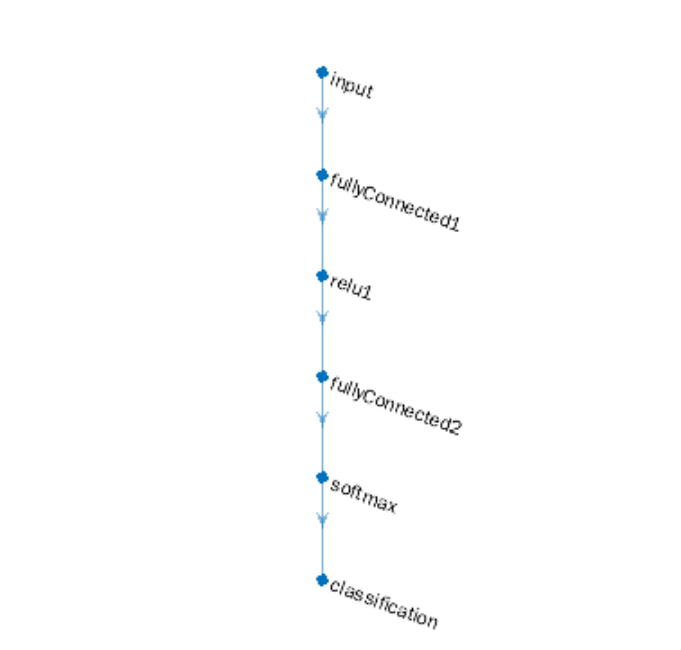
\includegraphics[scale = 0.4]{model.png}
    \caption{Netz Architektur}
\end{center}


\section{Aufgabe 1}

\subsection{Aufgabenstellung}
\\
1. Nutzen Sie die gegebene Matlab-Vorlage und laden Sie Bilder und Labels aus dem MNIST-Datensatz. Teilen Sie die Daten in Trainings- und
Validationsdaten auf.
\\
\subsection{Lösung}
\\
Die Daten werden aus der Neuronale Netze Toolbox Bibliothek geladen.\\
aus 1000 geladenen Daten werden 750 für Trainings-Daten und 250 für Validierungs-Daten verwendet

\\

\lstinputlisting{dataset.m}

\\

\section{Aufgabe2}
\\
\subsection{Aufgabenstellung}
\\
Erstellen Sie ein neuronales Netz zur Bildklassifizierung. Dieses sollte zum Beispiel aus einem Image input layer, einem Fully connected
layer, einem ReLU layer, einem weiteren Fully connected layer, einem Softmax layer und einem Classification layer (nur bei Verwendung der Funktion trainNetwork) bestehen. Achten Sie darauf, dass
das Softmax-Layer einen Vektor mit einer Länge entsprechend der zu
erkennenden Klassen benötigt, um die Klassifizierung zu ermöglichen.
Benutzen Sie den Befehl analyzeNetwork, um ihre Struktur auf Fehler
zu prüfen. Legen Sie dann die Hyperparameter für das Training fest.
\\
\subsection{Lösung}
\\
Prinzipiell geh es hier bei um die Netzwerkarchitektur, welche bereits in Abschnitt 2 erläutert.
\end{document}
